% % ============================================================
% %  3. DATA
% % ============================================================
% \chapter{Data}\label{sec:data}
% The analysis in this paper draws on two monthly time series sourced from Eurostat, covering Denmark and the EU27 over the period from December 2000 to March 2026. The former is the Harmonised Index of Consumer Prices (HICP), measured as the annual rate of change in percent \parencite{eurostat_hicp}. The latter is the monthly unemployment rate, expressed as a percentage of the labour force for both sexes and all ages, not seasonally adjusted \parencite{eurostat_unemployment}. The estimation sample is restricted to the common observation period beginning in December 2000 due to data availability constraints in the European inflation series.

% \begin{table}[h!]
% \centering
% \small
% \caption{Data sources. All series are retrieved directly from Eurostat.}
% \label{tab:data_sources}
% \begin{tabular*}{\textwidth}{@{\extracolsep{\fill}}lll}
% \hline \hline
% \rule{0pt}{12pt}\textbf{Series} & \textbf{Region} & \textbf{Definition} \\ [3pt]
% \hline
% \rule{0pt}{12pt}Unemployment rate & Denmark & Eurostat harmonised, Total, monthly \\ [3pt]
% \rule{0pt}{12pt}Unemployment rate & EU (27 countries) & Eurostat harmonised, Total, monthly \\ [3pt]
% \rule{0pt}{12pt}HICP rates of change & Denmark & Eurostat harmonised, not seas.\ adj., monthly \\ [3pt]
% \rule{0pt}{12pt}HICP rates of change & EU (27 countries) & Eurostat harmonised, not seas.\ adj., monthly \\ [3pt]
% \hline \hline
% \end{tabular*}
% \end{table}

% \section{Inspections of Raw Data}

% \paragraph{Looking for trend}
% Figure~\ref{fig:raw_data} shows the four unaltered series from December 2000 to March 2026. Danish and EU27 HICP inflation track each other closely over the sample period, remaining within 0 to 4 percent before surging to around 10 to 12 percent, in 2022 amid the post-COVID surge. The inflation levels have since then retreated toward pre-shock levels. Neither series displays a clear deterministic trend. Their apparent co-movement motivates the inclusion of EU27 HICP inflation as a predictor in the multivariate framework.

% Danish and EU27 unemployment display markedly different dynamics. EU27 unemployment follows a clear downward trend, peaking at 11 to 12 percent during the European sovereign debt crisis in 2012 and 2013 before declining steadily thereafter. Danish unemployment, by contrast, exhibits a roughly flat trend with a mild upward drift.

% \begin{figure}[H]
%     \centering
%     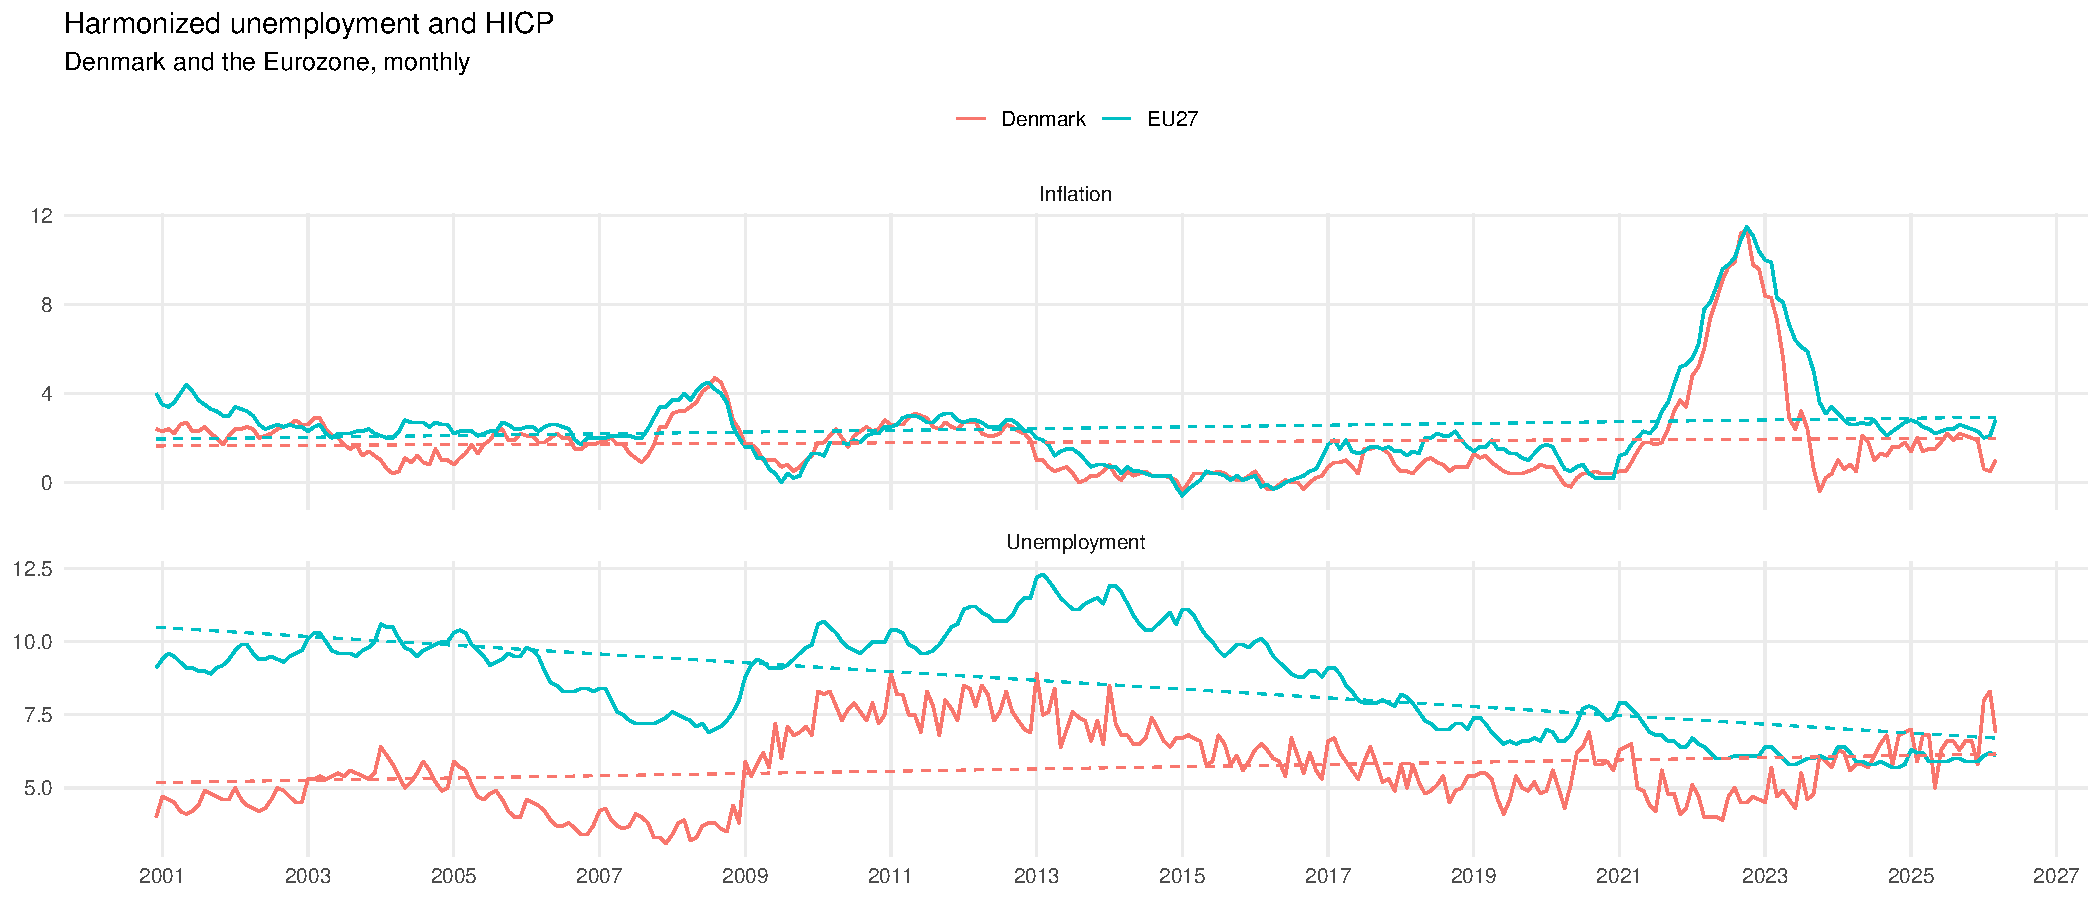
\includegraphics[width=1\linewidth]{billeder/facet_plot.pdf}
%     \caption{Faceted plot of European and Danish inflation and unemployment.}
%     \label{fig:raw_data}
% \end{figure}

% The time series plot in Figure~\ref{fig:raw_data} reveals the co-movement between Danish and EU27 inflation throughout the sample. Both series declined toward zero in the aftermath of the 2008 financial crisis, briefly turned negative around 2015, and surged sharply in 2021/22 before retreating afterwards. The EU27 series reached a slightly higher peak of approximately 12 percent compared to around 11 percent for Denmark, but the timing and shape of the shock are virtually indistinguishable. This close co-movement reflects Denmark's fixed exchange rate peg to the euro under ERM II and suggests that EU27 inflation may carry predictive information for Danish inflation. This motivates its inclusion as an additional predictor in our fourth forecasting model. 

% \paragraph{Initial look at the Phillips curve}
% The scatter plot reveals a weak negative relationship between Danish unemployment and Danish inflation over the sample period, consistent with the theoretical prediction of the Phillips curve. The fitted line slopes downward, suggesting that lower unemployment is on average associated with higher inflation. However, the relationship is far from tight. We see that the dispersion around the fitted line is substantial, and several observations with low unemployment are associated with very low or even negative inflation, while high inflation observations appear across the full range of unemployment rates. The post-COVID inflation surge is visible as a cluster of high inflation observations at relatively low unemployment levels in the upper left of the plot.

% \begin{figure}[H]
%     \centering
%     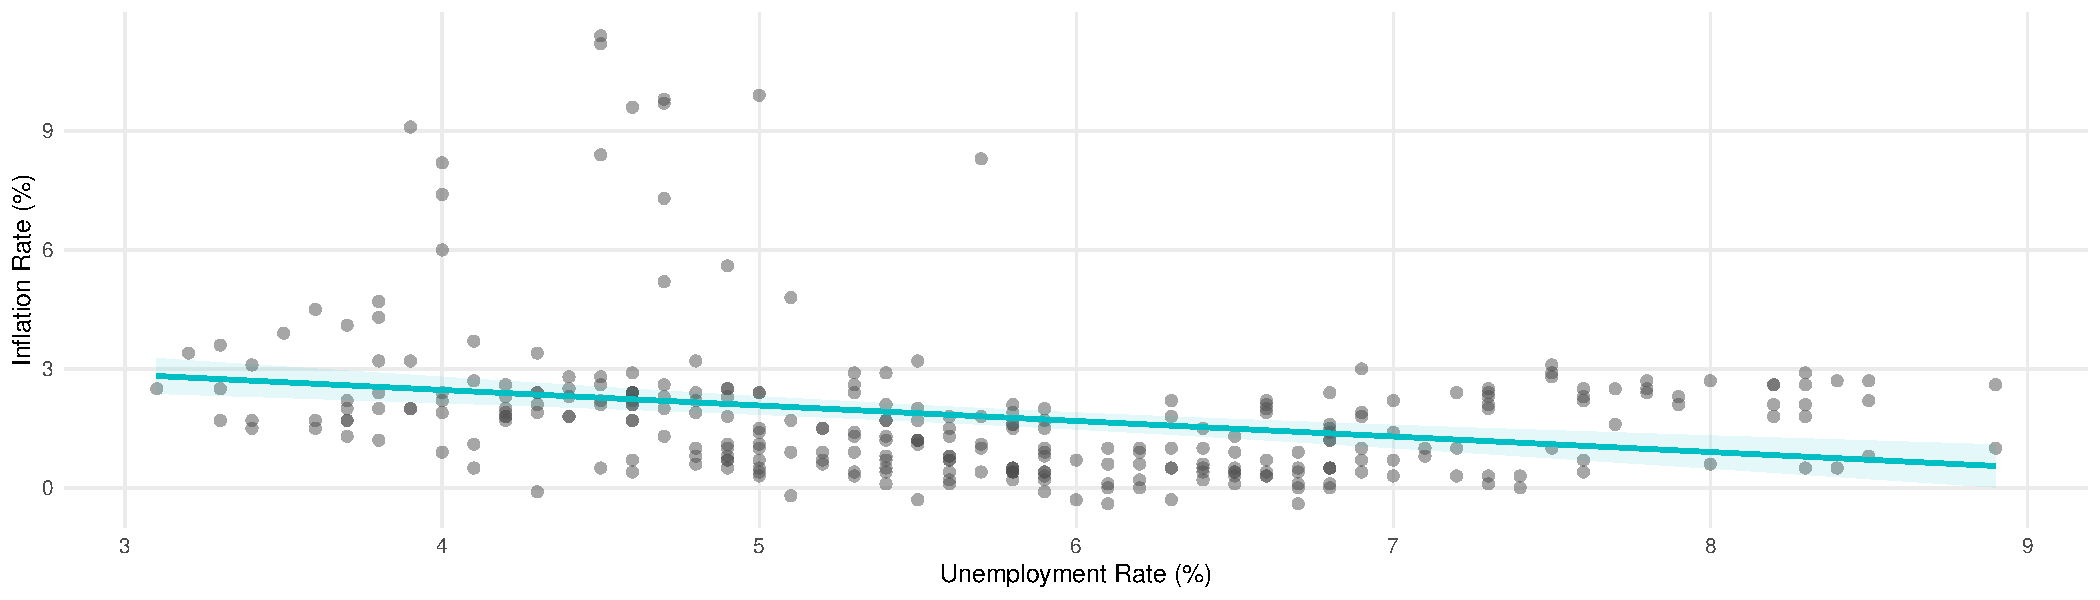
\includegraphics[width=0.75\textwidth]{billeder/phillips.pdf}
%     \caption{Scatter plot of Danish inflation against unemployment, with OLS fitted line.}
%     \label{fig:02_philips_curve_denmark}
% \end{figure}


% The scatter plot suggests that while a negative correlation exists between the two series, unemployment alone explains little of the variation in Danish inflation. Thus, we will later in this paper more formally assess whether unemployment retains predictive value for inflation.

% \paragraph{Looking for seasonality}
% The seasonal plots indicate some recurring seasonal variation in unemployment, particularly for the euro area, where unemployment tends to be higher in winter and lower during the summer months. The pattern is weaker for Danish unemployment. In contrast, inflation displays less systematic seasonality. The inflation plots are dominated by a few high-inflation years, suggesting that variation is driven more by macroeconomic shocks than by stable monthly seasonal patterns (See Appendix \ref{fig:index_seasonal_plot}).



% \paragraph{Testing for stationarity}
% Before estimating the forecasting models, we assess the stationarity properties of each series using the Augmented Dickey-Fuller (ADF) test and the KPSS test. The ADF test has non-stationarity as the null hypothesis, while the KPSS test has stationarity as the null hypothesis. The ACF and PACF plots, reported in Appendix~\ref{sec:appendix_acf_pacf}, serve as a graphical supplement, since we see slowly decaying autocorrelations it may indicate non-stationarity or remaining seasonal / autocorrelative dependence that our ARIMA models aim to capture.

% Table~\ref{tab:stationarity_levels} reports results for the series in levels. The inflation series, sourced directly as year-on-year rates of change, are already stationary transformations of the underlying price indices. Danish inflation is confirmed stationary by both tests. EU27 inflation yields mixed results at the levels stage, though this is not uncommon given the sharp but transitory nature of the 2022 inflation surge. Both unemployment series are non-stationary in levels according to both tests, consistent with what the time series plots suggest.

% \begin{table}[H]
% \centering
% \small
% \caption{Stationarity tests}
% \label{tab:stationarity_levels}
% \begin{tabular*}{\textwidth}{@{\extracolsep{\fill}}lcccc}
% \hline \hline
% \rule{0pt}{12pt}\textbf{Variable} & \textbf{ADF p-value} & \textbf{ADF conclusion} & \textbf{KPSS p-value} & \textbf{KPSS conclusion} \\ [3pt]
% \hline
% \rule{0pt}{12pt}Danish inflation, level      & $<0.01$ & Stationary     & $>0.10$ & Stationary     \\ [3pt]
% \rule{0pt}{12pt}EU27 inflation, level        & $0.022$ & Stationary     & $>0.10$ & Stationary \\ [3pt]
% \rule{0pt}{12pt}Danish unemployment          & $0.821$ & Non-stationary & $0.012$ & Non-stationary \\ [3pt]
% \rule{0pt}{12pt}EU27 unemployment            & $0.827$ & Non-stationary & $<0.01$ & Non-stationary \\ [3pt]
% \hline \hline
% \end{tabular*}
% \end{table}

% The unemployment series are therefore transformed using first differences, $\Delta y_t = y_t - y_{t-1}$, prior to estimation. Seasonal differencing was also considered due to indications of annual dependence in the seasonal plots and ACFs; however, first differencing provided clearer evidence of stationarity, and any remaining seasonal dynamics are instead addressed at the modelling stage. Table~\ref{tab:stationarity_tests} confirms that all transformed series are stationary, and the series used in the models are specified accordingly.

% \begin{table}[H]
% \centering
% \small
% \caption{Stationarity tests for variables used in the models}
% \label{tab:stationarity_tests}
% \begin{tabular*}{\textwidth}{@{\extracolsep{\fill}}lcccc}
% \hline \hline
% \rule{0pt}{12pt}\textbf{Variable} & \textbf{ADF p-value} & \textbf{ADF conclusion} & \textbf{KPSS p-value} & \textbf{KPSS conclusion} \\ [3pt]
% \hline
% \rule{0pt}{12pt}Danish inflation, level          & $<0.01$ & Stationary & $>0.10$ & Stationary \\ [3pt]
% \rule{0pt}{12pt}EU27 inflation, level            & $0.022$ & Stationary & $>0.10$ & Stationary \\ [3pt]
% \rule{0pt}{12pt}Danish unemployment, first diff. & $<0.01$ & Stationary & $>0.10$ & Stationary \\ [3pt]
% \rule{0pt}{12pt}EU27 unemployment, first diff.   & $<0.01$ & Stationary & $>0.10$ & Stationary \\ [3pt]
% \hline \hline
% \end{tabular*}
% \end{table}

% The marginal shift in the EU27 inflation results between the two tables reflects that the test statistics for this borderline series are sensitive to lag specification and the post-surge observations included; taken together, the evidence supports treating it as stationary in levels. With stationarity established for all model inputs, we proceed to model specification and estimation.

% \paragraph{Structural break test (QLR)}\label{sec:QLR}
% To test for structural breaks in Danish inflation, we apply the Quandt Likelihood Ratio (QLR) test. The test searches over candidate break dates within the central 85 percent of the sample and identifies the date with the highest F-statistic. The sup-F statistic of 73.03 is highly significant ($p < 0.001$), leading us to reject the null hypothesis of parameter stability. The supremum is attained in September 2021, corresponding to the peak of the post-COVID inflation surge. Since year-on-year comparisons become mechanically distorted from April 2021 due to the COVID-19 price trough of April 2020, we set the training cutoff at that date to exclude the full abnormal episode from parameter estimation.

% The result motivates the estimation strategy in the following section: rather than including break dummies, we exclude the COVID period from the estimation window entirely and condition the model state on the full series afterwards. As a complementary approach, the GETS model in Section~\ref{sec:methodology} includes a surge dummy in its estimation window. 

% \begin{figure}[H]
%     \centering
%     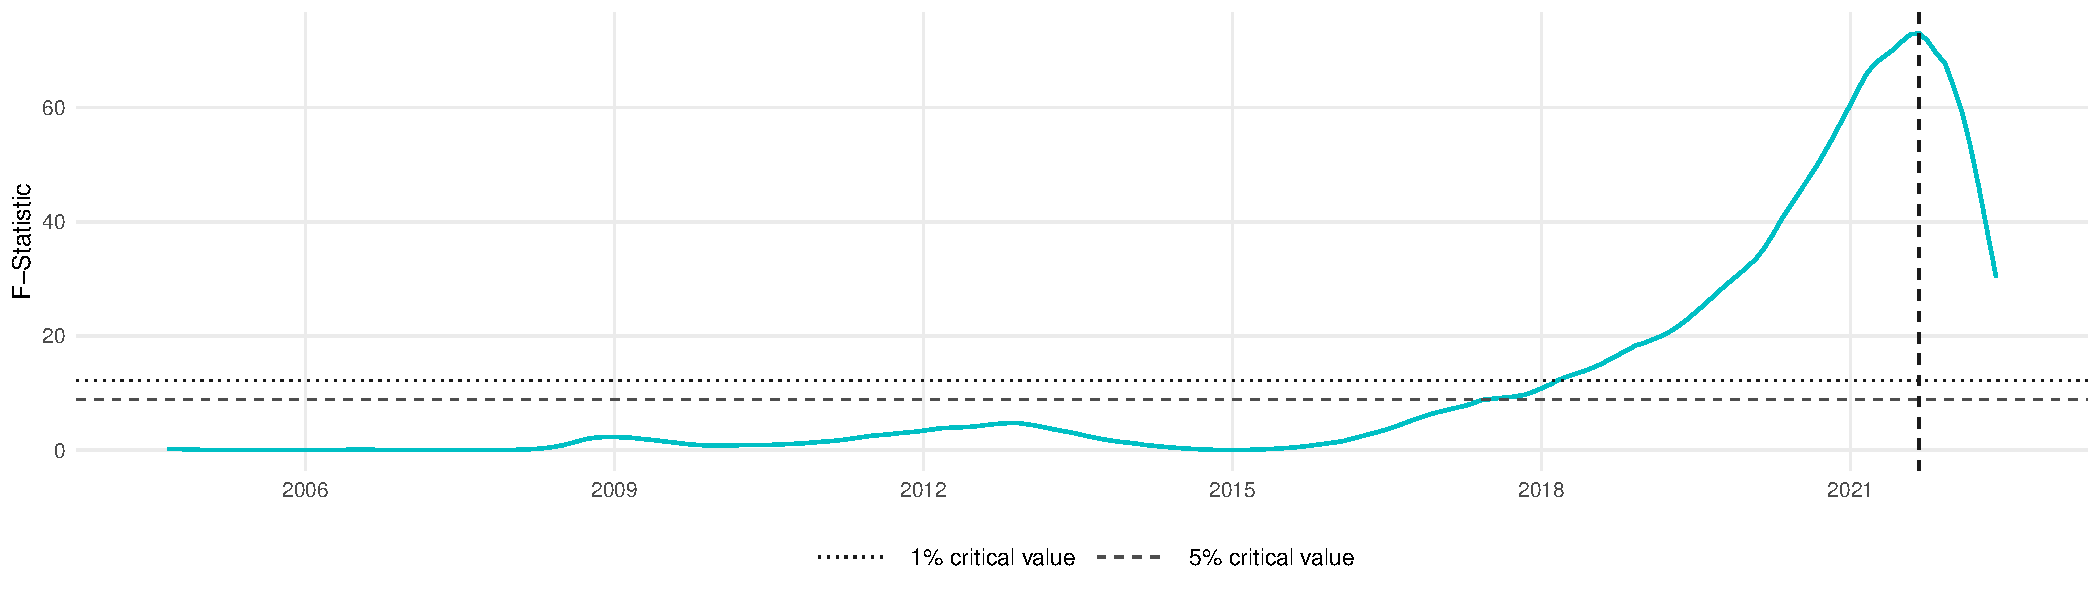
\includegraphics[width=\linewidth]{billeder/qlr.pdf}
%     \caption{QLR supremum F-statistic. Vertical line marks the estimated break date (September 2021).}
%     \label{fig:05_struc_break_test}
% \end{figure}



% \section{Granger Causality}\label{sec:granger}

% % To motivate the inclusion of EU27 inflation as an external regressor (in addtion to the also performing the test and forecasting using danish unemployment),  we conduct Granger causality tests using \texttt{grangertest()} from the \texttt{lmtest} package, tested at lag orders 1--6. The null hypothesis is that $X$ does not Granger-cause $Y$.

% To assess which external regressors carry predictive content for Danish inflation beyond its own history, we conduct Granger causality tests using \texttt{grangertest()} from the \texttt{lmtest} package, with the null that $X$ does not Granger-cause $Y$, tested at lag orders 1--6.

% \begin{table}[H]
% \centering
% \small
% \caption{Granger causality tests: $p$-values at lag orders 1--6.}
% \label{tab:granger}
% \begin{tabular*}{\textwidth}{@{\extracolsep{\fill}}lcccccc}
% \hline \hline
% \rule{0pt}{12pt} \textbf{Null hypothesis} & \textbf{Lag 1} & \textbf{Lag 2} & \textbf{Lag 3} & \textbf{Lag 4} & \textbf{Lag 5} & \textbf{Lag 6} \\ [3pt]
% \hline
% \rule{0pt}{12pt}EU27 infl.\ $\not\to$ DK infl.\ & 0.001 & 0.000 & 0.000 & 0.001 & 0.003 & 0.003 \\ [3pt]
% \rule{0pt}{12pt}EU27 unemp.\ $\not\to$ DK infl.\ & 0.715 & 0.648 & 0.865 & 0.957 & 0.972 & 0.986 \\ [3pt]
% \rule{0pt}{12pt}DK unemp.\ $\not\to$ DK infl.\ & 0.621 & 0.849 & 0.899 & 0.604 & 0.793 & 0.866 \\ [3pt]
% \hline \hline
% \end{tabular*}
% \end{table}

% EU27 inflation strongly Granger-causes Danish inflation across all lag orders ($p < 0.01$), consistent with Denmark's ERM~II peg and deep trade integration with the euro area. By contrast, neither EU27 nor Danish unemployment shows any predictive power for Danish inflation at any lag (all $p > 0.60$), providing no empirical support for a domestic or imported Phillips curve channel. These findings directly motivate Model~4, which incorporates EU27 inflation as an external regressor. As EU27 unemployment shows no predictive content for Danish inflation at any tested lag order, it is excluded from the subsequent modelling.

% ============================================================
%  3. DATA
% ============================================================
\chapter{Data}\label{sec:data}
The analysis in this paper draws on two monthly time series sourced from Eurostat, covering Denmark and the EU27 over the period from December 2000 to March 2026. The former is the Harmonised Index of Consumer Prices (HICP), measured as the annual rate of change in percent \parencite{eurostat_hicp}. The latter is the monthly unemployment rate, expressed as a percentage of the labour force for both sexes and all ages, not seasonally adjusted \parencite{eurostat_unemployment}. The estimation sample is restricted to the common observation period beginning in December 2000 due to data availability constraints in the European inflation series.

\begin{table}[h!]
\centering
\small
\caption{Data sources. All series are retrieved directly from Eurostat.}
\label{tab:data_sources}
\begin{tabular*}{\textwidth}{@{\extracolsep{\fill}}lll}
\hline \hline
\rule{0pt}{12pt}\textbf{Series} & \textbf{Region} & \textbf{Definition} \\ [3pt]
\hline
\rule{0pt}{12pt}Unemployment rate & Denmark & Eurostat harmonised, Total, monthly \\ [3pt]
\rule{0pt}{12pt}Unemployment rate & EU (27 countries) & Eurostat harmonised, Total, monthly \\ [3pt]
\rule{0pt}{12pt}HICP rates of change & Denmark & Eurostat harmonised, not seas.\ adj., monthly \\ [3pt]
\rule{0pt}{12pt}HICP rates of change & EU (27 countries) & Eurostat harmonised, not seas.\ adj., monthly \\ [3pt]
\hline \hline
\end{tabular*}
\end{table}

\section{Inspections of Raw Data}

\paragraph{Looking for trend}
Figure~\ref{fig:raw_data} shows the four unaltered series from December 2000 to March 2026. Danish and EU27 HICP inflation track each other closely over the sample period, remaining within 0 to 4 percent before surging to around 10 to 12 percent across the two series in 2022 amid the post-COVID surge. The inflation levels have since retreated toward pre-shock levels. Neither series displays a clear deterministic trend. Their apparent co-movement motivates the inclusion of EU27 HICP inflation as a predictor in the multivariate framework.

Danish and EU27 unemployment display markedly different dynamics. EU27 unemployment follows a clear downward trend, peaking at 11 to 12 percent during the European sovereign debt crisis in 2012 and 2013 before declining steadily thereafter. Danish unemployment, by contrast, exhibits a roughly flat trend with a mild upward drift.

\begin{figure}[H]
    \centering
    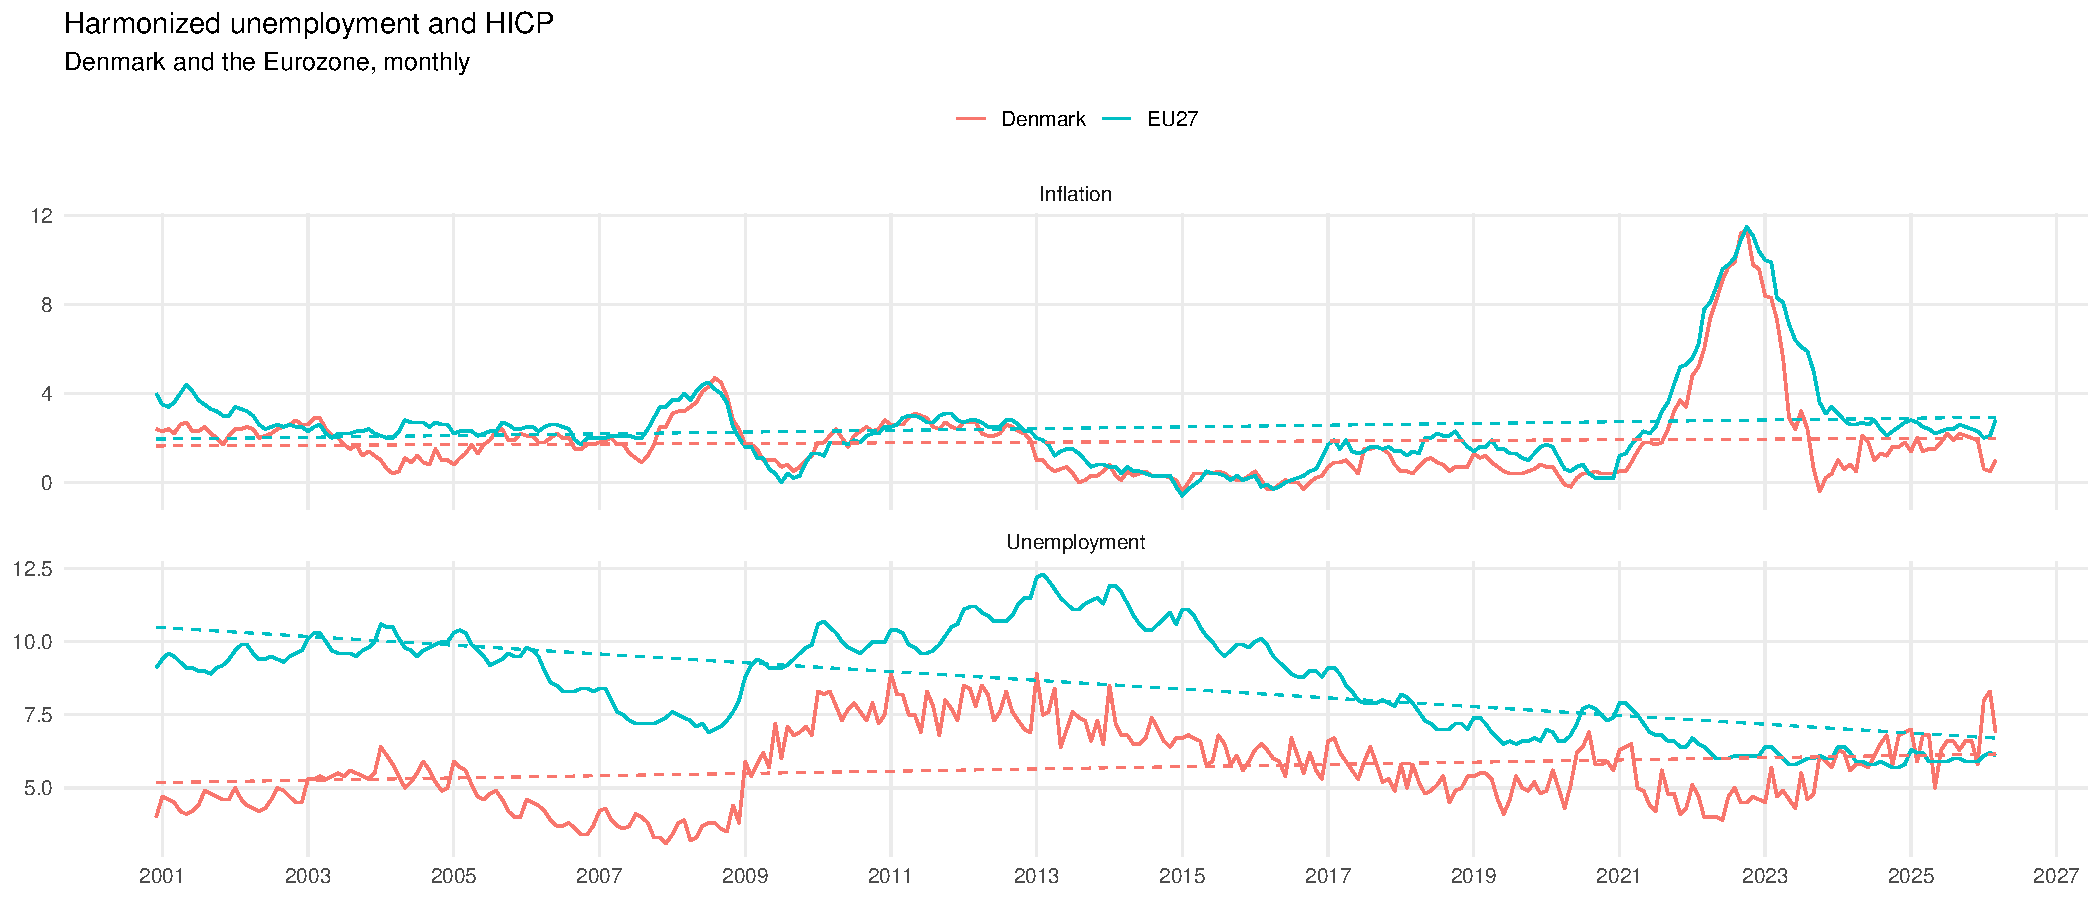
\includegraphics[width=1\linewidth]{billeder/facet_plot.pdf}
    \caption{Faceted plot of European and Danish inflation and unemployment.}
    \label{fig:raw_data}
\end{figure}

The time series plot in Figure~\ref{fig:raw_data} reveals the co-movement between Danish and EU27 inflation throughout the sample. Both series declined toward zero in the aftermath of the 2008 financial crisis, briefly turned negative around 2015, and surged sharply in 2021/22 before retreating afterwards. The EU27 series reached a slightly higher peak of approximately 12 percent compared to around 11 percent for Denmark, but the timing and shape of the shock are closely aligned. This close co-movement reflects Denmark's fixed exchange rate peg to the euro under ERM II and suggests that EU27 inflation may carry predictive information for Danish inflation. This motivates its inclusion as an additional predictor in our fourth forecasting model.

\paragraph{Examining the Phillips curve}
The scatter plot reveals a weak negative relationship between Danish unemployment and Danish inflation over the sample period, consistent with the theoretical prediction of the Phillips curve. The fitted line slopes downward, suggesting that lower unemployment is on average associated with higher inflation. However, the relationship is far from tight. We see that the dispersion around the fitted line is substantial, and several observations with low unemployment are associated with very low or even negative inflation, while high inflation observations appear across the full range of unemployment rates. The post-COVID inflation surge is visible as a cluster of high inflation observations at relatively low unemployment levels in the upper left of the plot.

\begin{figure}[H]
    \centering
    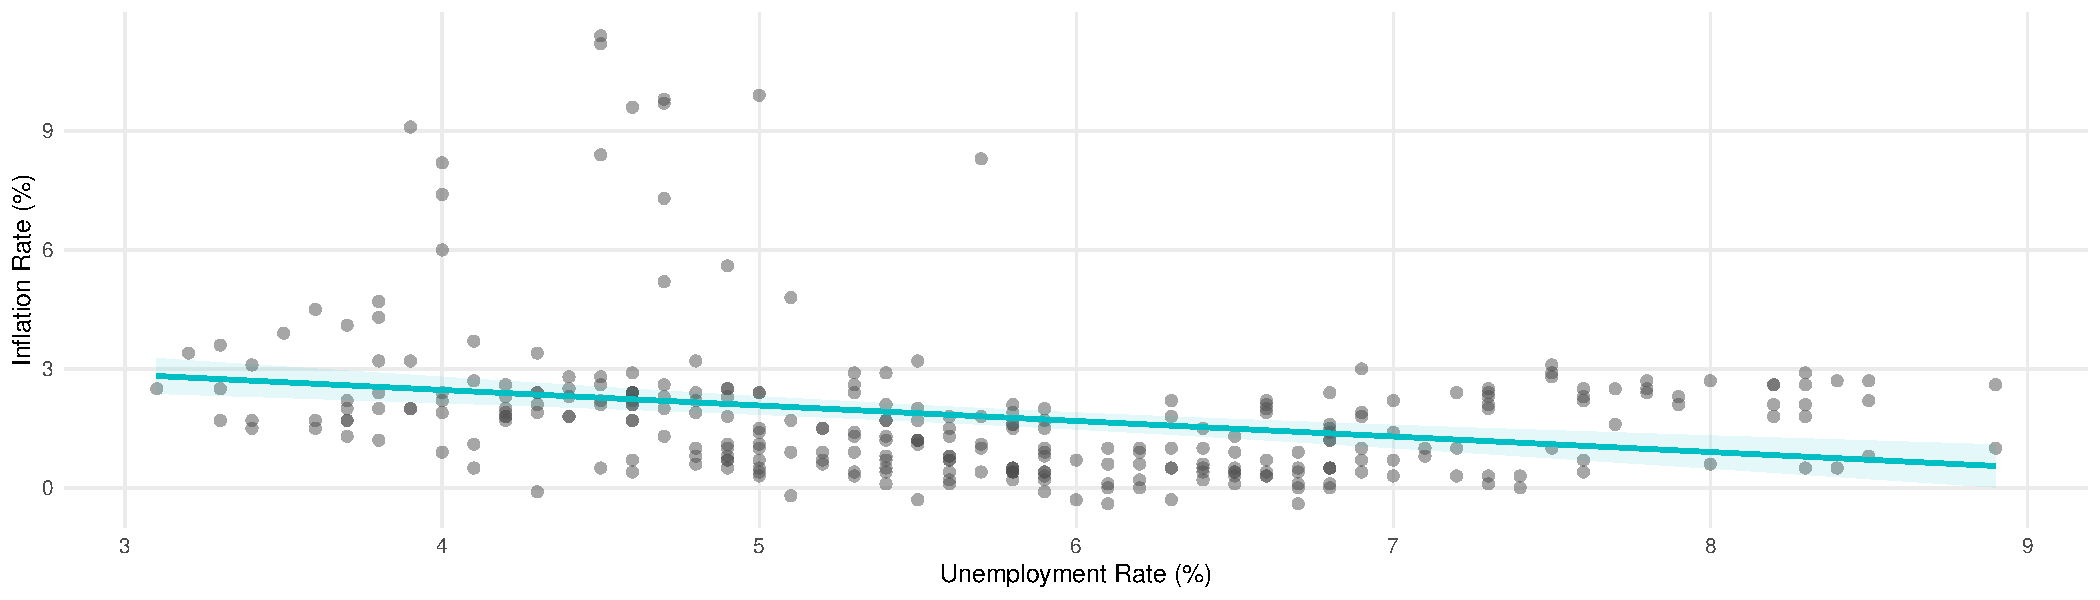
\includegraphics[width=0.75\textwidth]{billeder/phillips.pdf}
    \caption{Scatter plot of Danish inflation against unemployment, with OLS fitted line.}
    \label{fig:02_philips_curve_denmark}
\end{figure}

The scatter plot suggests that while a negative correlation exists between the two series, unemployment alone explains little of the variation in Danish inflation. Thus, we will later in this paper more formally assess whether unemployment retains predictive value for inflation.

\paragraph{Looking for seasonality}
The seasonal plots indicate some recurring seasonal variation in unemployment, particularly for the euro area, where unemployment tends to be higher in winter and lower during the summer months. The pattern is weaker for Danish unemployment. In contrast, inflation displays less systematic seasonality. The inflation plots are dominated by a few high-inflation years, suggesting that variation is driven more by macroeconomic shocks than by stable monthly seasonal patterns (see Appendix \ref{fig:index_seasonal_plot}).

\paragraph{Testing for stationarity}
Before estimating the forecasting models, we assess the stationarity properties of each series using the Augmented Dickey-Fuller (ADF) test and the KPSS test. The ADF test has non-stationarity as the null hypothesis, while the KPSS test has stationarity as the null hypothesis. The ACF and PACF plots, reported in Appendix~\ref{sec:appendix_acf_pacf}, serve as a graphical supplement, since we see slowly decaying autocorrelations, it may indicate non-stationarity or remaining seasonal / autocorrelative dependence that our ARIMA models aim to capture.

Table~\ref{tab:stationarity_levels} reports results for the series in levels. The inflation series, sourced directly as year-on-year rates of change, are already stationary transformations of the underlying price indices. Danish inflation is confirmed stationary by both tests. EU27 inflation yields mixed results at the levels stage, though this is not uncommon given the sharp but transitory nature of the 2022 inflation surge. Both unemployment series are non-stationary in levels according to both tests, consistent with what the time series plots suggest.

\begin{table}[H]
\centering
\small
\caption{Stationarity tests}
\label{tab:stationarity_levels}
\begin{tabular*}{\textwidth}{@{\extracolsep{\fill}}lcccc}
\hline \hline
\rule{0pt}{12pt}\textbf{Variable} & \textbf{ADF p-value} & \textbf{ADF conclusion} & \textbf{KPSS p-value} & \textbf{KPSS conclusion} \\ [3pt]
\hline
\rule{0pt}{12pt}Danish inflation, level      & $<0.01$ & Stationary     & $>0.10$ & Stationary     \\ [3pt]
\rule{0pt}{12pt}EU27 inflation, level        & $0.022$ & Stationary     & $>0.10$ & Stationary \\ [3pt]
\rule{0pt}{12pt}Danish unemployment          & $0.821$ & Non-stationary & $0.012$ & Non-stationary \\ [3pt]
\rule{0pt}{12pt}EU27 unemployment            & $0.827$ & Non-stationary & $<0.01$ & Non-stationary \\ [3pt]
\hline \hline
\end{tabular*}
\end{table}

The unemployment series are therefore transformed using first differences, $\Delta y_t = y_t - y_{t-1}$, prior to estimation. Seasonal differencing was also considered due to indications of annual dependence in the seasonal plots and ACFs; however, first differencing provided clearer evidence of stationarity, and any remaining seasonal dynamics are instead addressed at the modelling stage. Table~\ref{tab:stationarity_tests} confirms that all transformed series are stationary, and the series used in the models are specified accordingly.

\begin{table}[H]
\centering
\small
\caption{Stationarity tests after differencing}
\label{tab:stationarity_tests}
\begin{tabular*}{\textwidth}{@{\extracolsep{\fill}}lcccc}
\hline \hline
\rule{0pt}{12pt}\textbf{Variable} & \textbf{ADF p-value} & \textbf{ADF conclusion} & \textbf{KPSS p-value} & \textbf{KPSS conclusion} \\ [3pt]
\hline
\rule{0pt}{12pt}Danish inflation, level          & $<0.01$ & Stationary & $>0.10$ & Stationary \\ [3pt]
\rule{0pt}{12pt}EU27 inflation, level            & $0.022$ & Stationary & $>0.10$ & Stationary \\ [3pt]
\rule{0pt}{12pt}Danish unemployment, first diff. & $<0.01$ & Stationary & $>0.10$ & Stationary \\ [3pt]
\rule{0pt}{12pt}EU27 unemployment, first diff.   & $<0.01$ & Stationary & $>0.10$ & Stationary \\ [3pt]
\hline \hline
\end{tabular*}
\end{table}

With stationarity established for all model inputs, we proceed to model specification and estimation.

\paragraph{Testing for structural breaks (QLR)}\label{sec:QLR}
To test for structural breaks in Danish inflation, we apply the Quandt Likelihood Ratio (QLR) test. The test searches over candidate break dates within the central 85 percent of the sample and identifies the date with the highest F-statistic. The sup-F statistic of 73.03 is highly significant ($p < 0.001$), leading us to reject the null hypothesis of parameter stability. The supremum is attained in September 2021, corresponding to the peak of the post-COVID inflation surge (see Figure \ref{fig:05_struc_break_test}). Since year-on-year comparisons become mechanically distorted from April 2021 due to the COVID-19 price trough of April 2020, we set the cutoff date for the pre-surge sample at April 2021 to capture the full abnormal episode.

The result motivates the estimation strategy in the following section where we try to exclude the COVID period from the estimation window entirely and condition the model state on the full series afterwards. As a complementary approach, we include a surge dummy in the estimation window of the GETS model presented in Section~\ref{sec:dynregmodel} to investigate whether it provides additional explanatory value.

\begin{figure}[H]
    \centering
    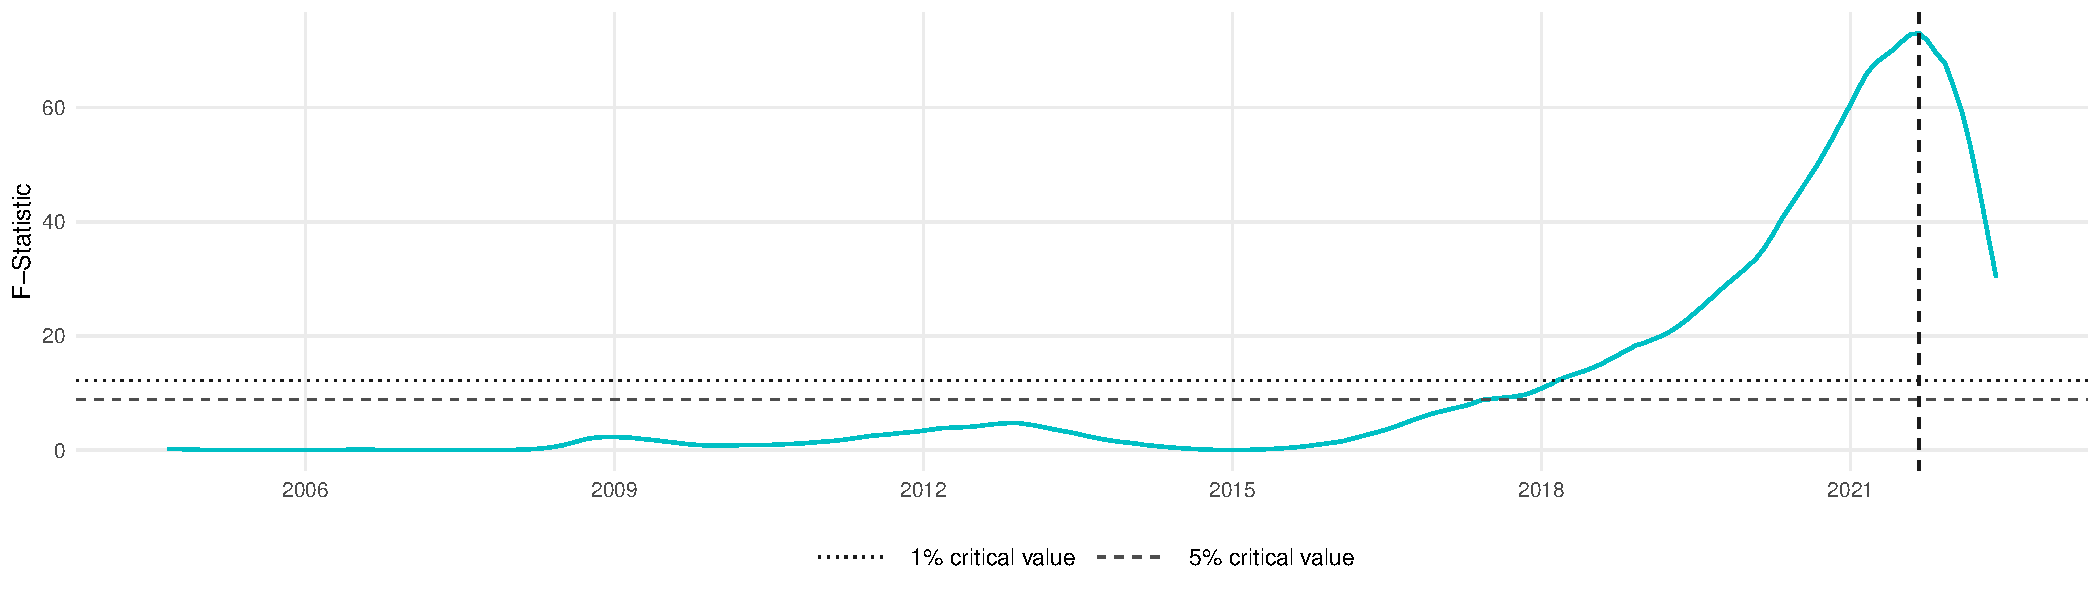
\includegraphics[width=\linewidth]{billeder/qlr.pdf}
    \caption{QLR supremum F-statistic. Vertical line marks the estimated break date (September 2021).}
    \label{fig:05_struc_break_test}
\end{figure}

\section{Granger Causality}\label{sec:granger}

To assess which external regressors carry predictive content for Danish inflation beyond its own history, we conduct Granger causality tests using \texttt{grangertest()} from the \texttt{lmtest} package, with the null hypothesis that $X$ does not Granger-cause $Y$, tested at lag orders 1--6.

\begin{table}[H]
\centering
\small
\caption{Granger causality tests: $p$-values at lag orders 1--6.}
\label{tab:granger}
\begin{tabular*}{\textwidth}{@{\extracolsep{\fill}}lcccccc}
\hline \hline
\rule{0pt}{12pt} \textbf{Null hypothesis} & \textbf{Lag 1} & \textbf{Lag 2} & \textbf{Lag 3} & \textbf{Lag 4} & \textbf{Lag 5} & \textbf{Lag 6} \\ [3pt]
\hline
\rule{0pt}{12pt}EU27 infl.\ $\not\to$ DK infl.\ & 0.001 & 0.000 & 0.000 & 0.001 & 0.003 & 0.003 \\ [3pt]
\rule{0pt}{12pt}EU27 unemp.\ $\not\to$ DK infl.\ & 0.715 & 0.648 & 0.865 & 0.957 & 0.972 & 0.986 \\ [3pt]
\rule{0pt}{12pt}DK unemp.\ $\not\to$ DK infl.\ & 0.621 & 0.849 & 0.899 & 0.604 & 0.793 & 0.866 \\ [3pt]
\hline \hline
\end{tabular*}
\end{table}

EU27 inflation strongly Granger-causes Danish inflation across all lag orders ($p < 0.01$), consistent with Denmark's ERM~II peg and deep trade integration with the euro area. By contrast, neither EU27 nor Danish unemployment shows any predictive power for Danish inflation at any lag (all $p > 0.60$), providing no empirical support for a Phillips curve channel. These findings directly motivate Model~4, which incorporates EU27 inflation as an external regressor. As EU27 unemployment shows no predictive content for Danish inflation at any tested lag order, it is excluded from the subsequent modelling.